\documentclass[conference]{IEEEtran}
\usepackage{amsmath,amssymb,amsfonts}
\usepackage{graphicx}
\usepackage{textcomp}
\usepackage{booktabs}
\usepackage{cite}
\usepackage{url}

\graphicspath{{./}{images/}{figures/}}

\begin{document}

\title{SCAATA: A Self Critiquing Autonomous Algorithmic Trading Agent with a Shared Risk Vocabulary}

\author{
\IEEEauthorblockN{R. Arzoo}
\IEEEauthorblockA{Bennett University, Greater Noida\\
201312, Uttar Pradesh, India\\
Email: E23CSEU2419@bennett.edu.in}
\and
\IEEEauthorblockN{G. Richa}
\IEEEauthorblockA{Bennett University, Greater Noida\\
201312, Uttar Pradesh, India\\
Email: E23CSEU2419@bennett.edu.in}
}

\maketitle

\begin{abstract}
Trading systems seldom announce their own failure. A rule based system cannot tell that its rules quit working. A reinforcement learning agent collects reward for years and never asks what risk paid for it. SCAATA looks back at what it just did. That review then changes how it learns next. One idea holds the design together. We call it the critique vocabulary. It has three risk terms. The first covers drawdown extension. The second covers entries taken into high volatility. The third covers losing positions held too long. Those three terms do four jobs. They shape the reward. They set the per expert loss in a regret bounded council. They act as fitness for strategies grown by genetic programming. They also score the devil's advocate counterfactual. So everything is measured in the same units. That has one useful consequence. The trained policy can be replayed over history. It then joins the council as just another expert. The rule that judges a scraped crossover now judges the policy too. Results come in three groups. An early study on six large cap technology stocks reported a median Sharpe near 1.1 against 0.6 for vanilla PPO. No code or saved output in this repository reproduces it, so we withdraw it. We then widen to nine stocks, nine walk forward folds, and five seeds, using vanilla recurrent PPO without the critique machinery. Across all five seeds it averages a Sharpe of 0.17 against 0.68 for buy and hold on the same windows, trailing by 0.51 in a fold clustered comparison and leading in one fold out of nine. We find no evidence of an edge over buy and hold, a rule based baseline, or a simple momentum heuristic. The third group is what broke. Hand tuned reward penalties taught the agent to stop trading. A differential Sharpe reward flipped its own risk preference above a measurable rate. Single seed feature tests disagreed wildly across tickers. A multi seed check traced most of that to noise. We report the failures beside the successes. They taught us more.
\end{abstract}

\begin{IEEEkeywords}
algorithmic trading, Proximal Policy Optimization, reinforcement learning, self critiquing agents, multiplicative weights, regret minimization, novelty detection, walk forward validation
\end{IEEEkeywords}

\section{Introduction}

Take a rule based trading system. Its logic is a fixed map from indicators to actions. A moving average crossover behaves impeccably inside the regime somebody tuned it on. Then the regime ends. Nothing in the design registers this. The rule keeps firing at full confidence through a calm tape and a collapsing one alike. It was never given any way to tell those apart.

Reinforcement learning was meant to be the cure. Frame trading as sequential decision making. Learn the policy from data. Throw away the hand coded rules. In practice the learned policy decays out of sample almost as fast as whatever it displaced. Give exploration no structural prior and it wastes most of its budget. It rediscovers things a junior analyst could have written down in an afternoon.

Structure has since been added in various places. MetaTrader \cite{niu2022metatrader} steadies early training with imitation learning and a meta policy that picks among strategies. The mixture of actors work \cite{cheng2024mot} runs several policies at once, so regime transitions hurt less. Neuro symbolic methods \cite{harini2023neurosymbolic} import domain priors to shrink the search space. None of them close one particular loop. The portfolio lives through something. That experience never reaches the policy update. Suppose the meta policy picks a bad strategy. Nothing carries that fact back into training, beyond the raw reward it already had.

Closing that loop is what SCAATA does. The mechanism we want to put forward is narrower than the system around it. It comes down to a single decision. Score everything in the same units.

\subsection{The Critique Vocabulary}

Three risk terms are defined over a rolling window of realized profit and loss. The first triggers when a drawdown deepens past a threshold. The second triggers when the agent opens a position while short term volatility runs hot against its own baseline. The third triggers when a losing position is held past a grace period. We call this triple the critique vocabulary. Section \ref{sec:vocab} gives the equations.

None of that is the interesting part. Risk shaped reward terms are old. They go back at least to Moody and Saffell's differential Sharpe ratio \cite{moody2001learning}. What matters is how the vocabulary is used. Inside SCAATA it is the only scoring language in the pipeline:

\begin{itemize}
\item it shapes the reward the reinforcement learning agent sees at every step;
\item it becomes the per expert loss that drives a multiplicative weights update over the strategy pool;
\item it is the fitness function that selects evolved candidate strategies;
\item it scores the counterfactual the devil's advocate agent constructs each round.
\end{itemize}

Four roles, one language. A component can move between them with nothing to translate. That is what lets us take the trained policy and replay it across history. We get its implied action sequence. We hand that to the expert council as just another entrant. From there the policy gains or sheds weight under one rule. It is the same rule that governs a crossover scraped off GitHub. Score your components in four separate currencies and none of this is available. That is the claim, not any individual penalty term.

\subsection{Literature Review}

Table \ref{tab:litreview} runs from the early value based methods to today's hybrids. The pattern is consistent. Each generation repairs one weakness and leaves the neighbouring ones alone. Jeong and Kim \cite{jeong2019dqn} put deep Q networks onto discrete trading decisions. Their in sample results looked good until a regime shifted underneath them. Th\'eate and Ernst \cite{theate2021drl} improved training stability. Drift in the return distribution still forced the value function back into retraining. Liu et al. gave us FinRL \cite{liu2020finrl}, then FinRL-Meta \cite{liu2022finrlmeta}. Both are useful infrastructure. Neither is a new learning mechanism, so non stationarity at the policy level goes untouched.

MetaTrader \cite{niu2022metatrader} pairs imitation learning with a strategy selecting meta policy. That does cut the noise of early exploration. But the selector never looks at how its chosen strategy actually performed. So when the whole pool is underwater at once, nothing says react. Ensembles help too. The mixture of actors work \cite{cheng2024mot} shows this. Its individual actors still update with no trajectory level risk reaching them. Neuro symbolic reinforcement learning \cite{harini2023neurosymbolic} writes symbolic knowledge into the objective. That buys interpretability and costs adaptability. It is a poor trade once market structure wanders past the encoded rules. Zhang's cluster based PPO variant \cite{zhang2026cluster} hits a related wall. Clusters fixed offline say nothing about a transition outside the categories drawn during clustering. Two surveys \cite{ozbayoglu2020survey,bai2024survey} catalogue the same three complaints. Sample inefficiency. Non stationarity. No path carrying realized portfolio risk back into the learning update.

For the expert council we went to the prediction with expert advice literature. Ensemble deep learning was the other option. Freund and Schapire \cite{freund1997decision} give the multiplicative weights update and its regret bound. Cesa-Bianchi and Lugosi \cite{cesabianchi2006prediction} give the fuller treatment. A learned gating network was the obvious alternative. We passed on it for one reason. It is not auditable. Each expert's cumulative regret can be written down as a number. Whether that regret grows sublinearly is something we can check. That is a falsifiable statement about the mechanism, not a hopeful one about returns.

\begin{table*}[t]
\caption{Summary of reinforcement learning approaches in algorithmic trading}
\label{tab:litreview}
\centering
\begin{tabular}{p{2.3cm}p{4.3cm}p{2.8cm}p{4.5cm}}
\toprule
\textbf{Paper} & \textbf{Core Contribution} & \textbf{Approach} & \textbf{Key Limitation} \\
\midrule
Jeong \& Kim \cite{jeong2019dqn} & Deep Q networks for financial trading decisions & DQN, value based RL & Poor generalization under regime shifts \\
Th\'eate \& Ernst \cite{theate2021drl} & Improved training stability for RL trading & DQN variants & Unstable out of sample performance \\
Liu et al. \cite{liu2020finrl} & Standardized DRL pipeline (FinRL) & PPO, DQN, A2C framework & No adaptive mechanism for non stationarity \\
Liu et al. \cite{liu2022finrlmeta} & Benchmark environments for RL trading & Simulation and evaluation framework & Infrastructure focus, not policy improvement \\
Niu et al. \cite{niu2022metatrader} & Meta policy selecting among multiple strategies & Meta RL and imitation learning & No trajectory level feedback \\
Cheng et al. \cite{cheng2024mot} & Mixture of actors for robust trading & Multi policy RL ensemble & No explicit risk feedback loop \\
Harini et al. \cite{harini2023neurosymbolic} & Symbolic knowledge integration with RL & Neuro symbolic RL & Limited adaptability beyond predefined rules \\
Zhang \cite{zhang2026cluster} & Cluster based PPO for regime aware trading & PPO with offline clustering & Static clusters, weak online adaptation \\
Mnih et al. \cite{mnih2015dqn} & Human level control via deep Q networks & DQN with experience replay & Not designed for financial non stationarity \\
Schulman et al. \cite{schulman2017ppo} & Clipped surrogate objective for stable updates & Proximal Policy Optimization & Sensitive to reward scaling \\
Moody \& Saffell \cite{moody2001learning} & Differential Sharpe ratio as an online reward & Direct reinforcement & First order approximation, sensitive to adaptation rate \\
Freund \& Schapire \cite{freund1997decision} & Multiplicative weights with a regret bound & Prediction with expert advice & Assumes bounded losses, carries no domain model \\
Hambly et al. \cite{hambly2023recent} & Mathematical treatment of RL in finance & Policy gradient and value based RL & Limited empirical validation \\
Jiang et al. \cite{jiang2017deep} & Deep RL for continuous portfolio rebalancing & CNN based online policy & No transaction costs, limited regime robustness \\
Liang et al. \cite{liang2018adversarial} & Adversarial training for robust portfolio RL & DRL with adversarial perturbation & Adversarial distribution may not match real shifts \\
Ozbayoglu et al. \cite{ozbayoglu2020survey} & Survey of deep learning in finance & Survey & Limited depth on RL specific trading \\
Bai et al. \cite{bai2024survey} & Comprehensive survey of RL in finance & Survey & Documents instability and overfitting \\
\textbf{SCAATA (ours)} & One shared risk vocabulary scoring the reward, the expert weights, the evolution fitness, and the counterfactual critique & Imitation learning, regret bounded expert council, novelty modulation, recurrent PPO & Addresses non stationarity and risk aware learning \\
\bottomrule
\end{tabular}
\end{table*}

\subsection{Research Problem and Objectives}

Reinforcement learning for trading lacks a closed loop. Realized portfolio risk never runs back to the policy update. Three gaps follow from that absence.

First, regimes shift and trained policies decay. The typical system keeps adapting as though its training distribution were permanent. Second, a step level reward describes one action. It says nothing about the risk profile of the trajectory around it. Third, and this one bothered us most, nothing puts the learner and the hand written baselines on a common footing. Ask a deployed system how far to trust its own policy this morning against a simple rule. It has no way to answer.

The objectives track those gaps. Build a critique vocabulary. Apply it unchanged to reward shaping, expert weighting, strategy evolution, and counterfactual reasoning. Make the policy answerable inside the same weighting system as every other signal source. Then test whether any of it improves risk adjusted performance, under walk forward backtesting with Sharpe as the primary metric. A fourth objective emerged during the work rather than before it. It mattered more than we expected. Build the machinery that separates a real effect from seed noise, then publish whatever that machinery concludes.

\section{Methodology}

Two loops make up SCAATA, drawn in Fig. \ref{fig:dualloop}. The outer loop holds the reinforcement learning side. That means market data, features, regime and novelty detection, and the recurrent PPO policy. The inner loop holds the multi agent side. It scrapes candidate strategies. A language model normalizes them. A genetic stage evolves new ones. The pool it refines feeds back out to the outer loop.

\begin{figure}[t]
\centering
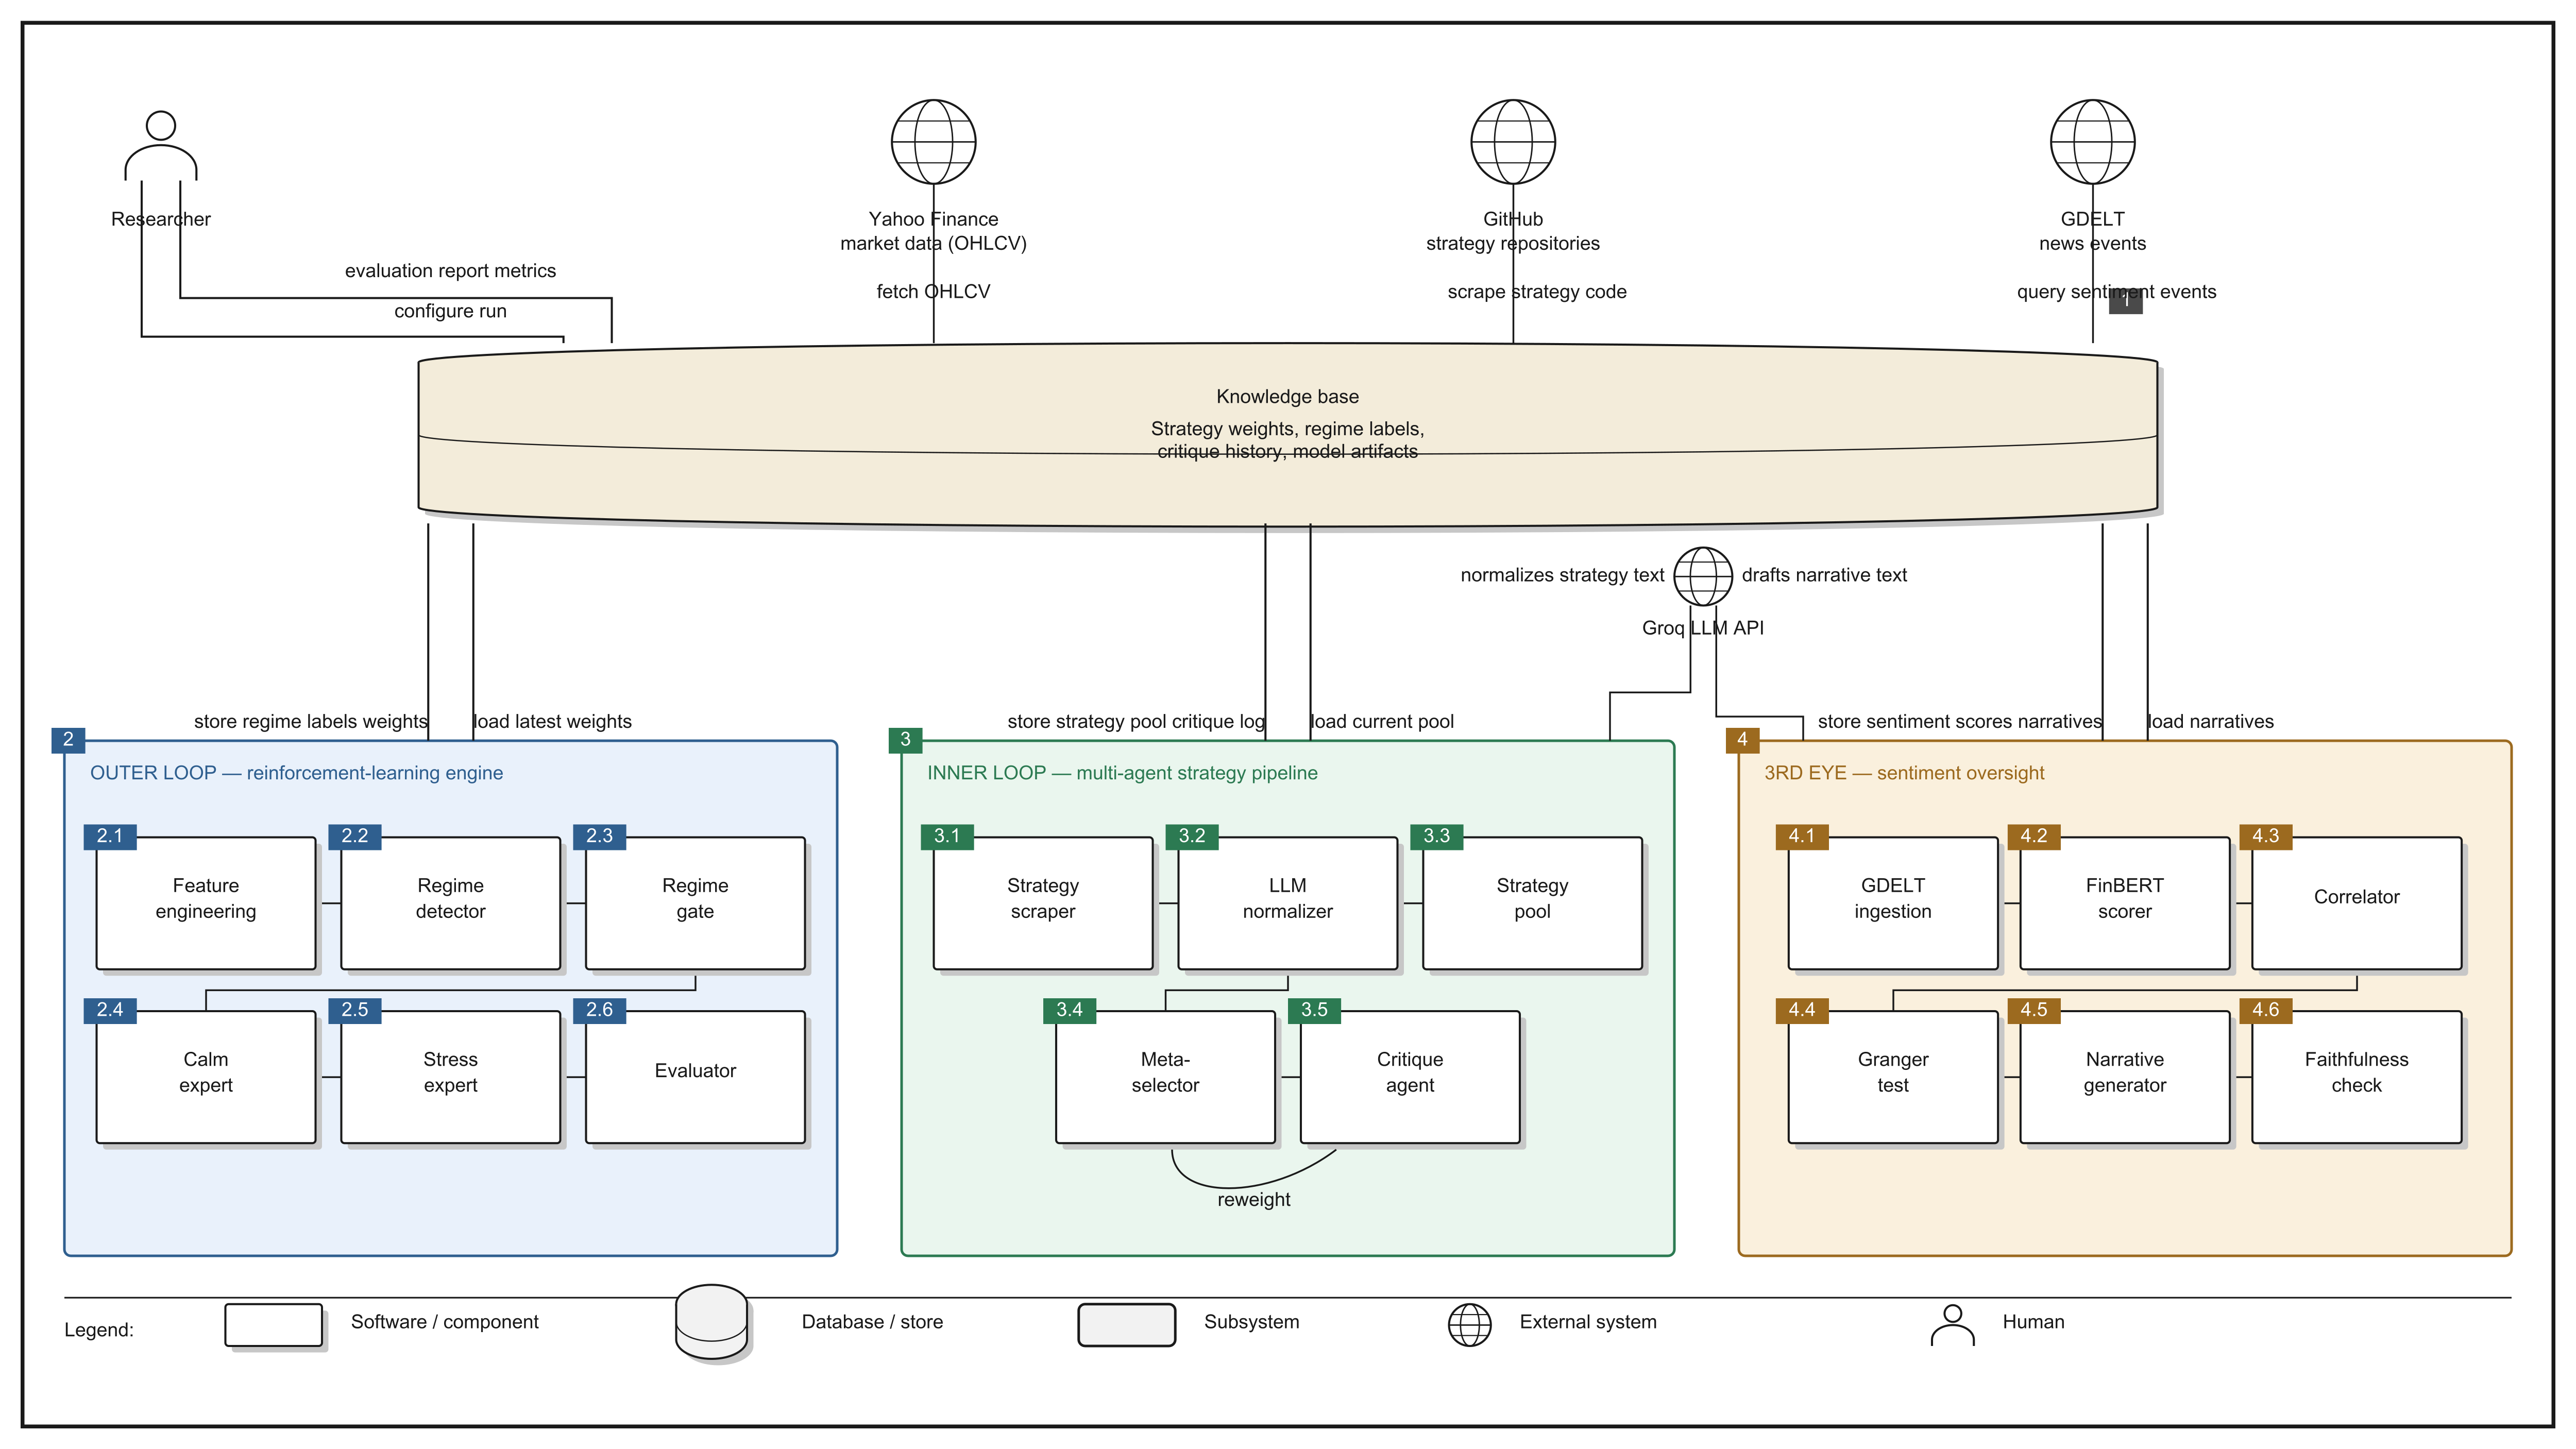
\includegraphics[width=0.48\textwidth]{fig_dual_loop.png}
\caption{Dual loop architecture. The outer loop trains and evaluates the RL policy against market data. The inner loop scrapes, normalizes, evolves, and critiques a pool of candidate strategies. Both loops read from and write to a shared knowledge base, which the outer loop's meta selector draws on directly.}
\label{fig:dualloop}
\end{figure}

\subsection{Outer Loop: Market Environment and Data}

Yahoo Finance supplies the daily OHLCV data. We forward fill missing values, then drop any row still carrying a gap. Rolling windows are the only thing features are built from, which keeps any feature at time $t$ from ever glimpsing data after $t$.

Feature engineering gives seven inputs per step. They are log return $r_t = \log(P_t / P_{t-1})$, moving averages of close over ten and fifty days, fourteen day RSI, ten day realized volatility, ten day momentum, and a thirty day volume average. The observed state is then
\begin{equation}
s_t = [r_t, MA_{10,t}, MA_{50,t}, RSI_t, \sigma_t, mom_t, V_{30,t}],
\label{eq:state}
\end{equation}
standardized on a rolling basis. Later phases append three optional columns. They are the meta selector's confidence in its top pick, a sentiment score, and a novelty score. Each one is opt in. Every earlier configuration therefore stays exactly reproducible.

The action space is $\mathcal{A} = \{\text{buy}, \text{hold}, \text{sell}\}$ and the base step reward is portfolio percentage change,
\begin{equation}
r_t = \frac{V_t - V_{t-1}}{V_{t-1}}.
\label{eq:basereward}
\end{equation}

Liquidity scales the transaction fees. The base rate is 0.1 percent. We multiply it by the ratio of thirty day average volume to current session volume. The result is capped between 0.5 and 5 times base. A hard stop loss liquidates any position that moves two percent against its entry. Execution charges a fixed penalty.

Both loops read from and write to a shared knowledge base. It holds every strategy the system knows about. An evaluator scores each one against market data in risk adjusted terms. Persistent underperformers lose weight for future sampling. Section \ref{sec:council} covers how that down weighting works. It no longer resembles the binary rule we started with.

\subsection{Inner Loop: Scraping, Normalization, and Evolution}

Candidate strategies come from public GitHub repositories. Keyword queries retrieve them, covering momentum, mean reversion, and crossover logic. We then filter on trading keyword density and deduplicate by hash. Whatever survives goes to a language model. It normalizes each file into a common $\text{strategy}(df)$ function returning integer signals in $\{-1, 0, 1\}$. Every strategy $\pi_i : \mathcal{S} \rightarrow \mathcal{A}$ sees the same feature set as the RL agent.

The original design stopped there. That imposes a ceiling. The pool can only hold code somebody already wrote. So we added a genetic programming stage \cite{koza1992genetic}. It grows fresh candidates straight out of the feature columns. Shallow rule trees get mutated and crossed. Each one compiles to a literal $\text{strategy}(df)$ source string. That string honours the existing pool contract without modification. We needed no new backtest engine and no language model call per candidate.

Two design choices here deserve saying out loud. Getting them wrong is a category error, not a tuning mistake. Start with the moving averages. They are absolute and price scaled. A 150 dollar stock and a 3000 dollar stock cannot share one fixed threshold. So those two features only appear in pairwise conditions against each other. That is a scale invariant crossover check. They never sit beside a numeric constant. Threshold conditions are reserved for the bounded features: return, momentum, RSI, volatility. The second choice is a depth cap of three. Even three conditions hold enough free thresholds to fit noise across a few thousand rows. Overfitting risk then climbs faster than a two and a half year test window can validate away.

Fitness averages across every available ticker rather than scoring per ticker. That makes life harder for a rule that memorised one idiosyncratic price path. Evolution selects on in sample fitness. The ranking returned to callers uses held out validation fitness instead. Being lucky in sample therefore earns a candidate nothing. We report the gap between those two numbers per candidate. It is the honest tell for overfitting.

\subsection{The Critique Vocabulary}
\label{sec:vocab}

A step level reward tells you whether one action made money. It says nothing about whether the sequence around it was accumulating danger. Picture two trades with identical per step reward. One was entered calmly. One chased a spike. Their risk is nothing alike. A policy trained on step reward alone cannot tell them apart.

Reviews in SCAATA run over a rolling window of $W = 20$ trading days. That is roughly one trading month. It is long enough for single day noise to average out. It is short enough that the agent reacts inside a quarter. We picked the number, we did not derive it. Section \ref{sec:limitations} is candid about what stays untested as a result.

Three quantities are tracked causally, meaning each uses only data available up to the current step. A drawdown extension penalty fires once running drawdown exceeds five percent,
\begin{equation}
\phi_{dd}(t) = \max\!\big(0,\ DD(t) - 0.05\big),
\label{eq:phidd}
\end{equation}
where $DD(t)$ is drawdown from the trailing peak. A volatility chasing penalty fires when the agent opens a position while short term volatility is elevated against its own baseline,
\begin{equation}
\phi_{vol}(t) = \max\!\Big(0,\ \frac{\sigma_{5}(t)}{\sigma_{30}(t)} - 1\Big),
\label{eq:phivol}
\end{equation}
using a five day window against a thirty day baseline. A prolonged holding penalty fires once a losing position has been held past a five day grace period,
\begin{equation}
\phi_{hold}(t) = \max\!\big(0,\ h(t) - 5\big) \cdot \mathbb{1}[\text{PnL}(t) < 0],
\label{eq:phihold}
\end{equation}
where $h(t)$ counts days the position has been open.

These combine into a shaped reward,
\begin{equation}
r'_t = r_t - \lambda_{dd}\,\phi_{dd}(t) - \lambda_{vol}\,\phi_{vol}(t) - \lambda_{hold}\,\phi_{hold}(t).
\label{eq:shaped}
\end{equation}

Provenance deserves precision here. The original design named the three penalties by role. It never wrote down a closed form for any of them. Equations \ref{eq:phidd} through \ref{eq:phihold} are our operationalization of that prose. We are not reproducing somebody else's equation. Taken individually, none of these terms is a contribution.

A second form of the same three terms sits beside the live per step tracker. It is vectorized and computed after the fact, over a finished trajectory slice. The expert council consumes that version. So do the evolution fitness function and the devil's advocate. Keeping both forms is a small engineering detail. It is also what makes the vocabulary portable between roles.

\subsection{The Expert Council}
\label{sec:council}

One binary rule used to govern the strategy pool. If the trailing window came back net negative, halve the weight of whatever got picked most often. The rule works in a narrow sense. Weight does move in the right direction. But it says nothing about magnitude. It says nothing about cause. And it guarantees nothing at all.

We replaced it with the standard prediction with expert advice update \cite{freund1997decision,cesabianchi2006prediction}. Every pooled strategy becomes an expert. Each round expert $i$ takes a loss $\ell_i$. Its weight then moves multiplicatively,
\begin{equation}
w_i^{(t+1)} \propto w_i^{(t)} \exp\!\big(-\eta\,\tilde{\ell}_i^{(t)}\big),
\label{eq:hedge}
\end{equation}
where $\tilde{\ell}$ denotes the loss min max normalized across experts within the round. Normalization matters here. A return based loss and a penalty based loss have wildly different raw scales. Only the relative ranking within a round is meaningful. The learning rate follows the textbook tuning
\begin{equation}
\eta = \sqrt{8 \ln N / T},
\label{eq:eta}
\end{equation}
which gives the $O(\sqrt{T \ln N})$ worst case regret bound against the best single expert in hindsight.

Loss is where the critique vocabulary enters. Calling direction correctly is not enough to score well. We replay the trailing window as though expert $i$ had been followed alone. Then we score that trajectory with the same window level report that drives reward shaping. Loss is the negative of window return plus total penalty. So an expert can get direction right through a reckless, deeply drawn down path. It then eats the penalty the reinforcement learning agent would eat for the same behaviour. An expert also cannot game this by refusing to trade. Dodging every penalty trigger still leaves nothing on the return side.

A projection with a floor puts weights back on the probability simplex. That deprioritizes an expert rather than deleting it mid run. The projection is trickier than it looks. Section \ref{sec:negative} explains why the obvious implementation is wrong.

We report cumulative regret per expert as an explicit number. That gives a falsifiable check on the mechanism itself. Growth should look roughly like $\sqrt{T \ln N}$, not linear in $T$. We test that.

\subsection{The Novelty Score}

The council's other problem is knowing when to forget. Two months of track record is informative while a market holds still. Once it moves, that record misleads. The original design would have used a branch on a discrete regime label. Something like a test for whether the current regime equals crisis. Discrete labels break down at the moment you need them most. A genuinely unfamiliar condition need not land in any bucket that existed when the buckets were drawn.

So our score is continuous. We compute it two independent ways. The first is a rolling Mahalanobis distance \cite{mahalanobis1936generalized}. It compares today's feature vector against the mean and covariance of the sixty days before it. The chi square survival function maps that into $[0,1]$. Treat the result as a ranking signal, not a calibrated probability. Daily returns are fat tailed, so the normality assumption underneath does not hold. The second method is a rolling discriminator. A logistic classifier is refit periodically to separate recent window rows from historical ones. Its predicted probability that a row is recent becomes the novelty score. Its own held out AUC gates it. A few features over a short window will happily produce an overfit model that says nothing. Below an AUC of 0.55 we discard the score.

Novelty enters the council in two separable ways. It multiplies the learning rate,
\begin{equation}
\eta_t = \eta \,\big(1 + \kappa \, \nu_t\big),
\label{eq:etanovelty}
\end{equation}
so the council discards stale performance faster when the environment is moving. Novelty also feeds an additive log prior. That prior nudges weight toward the sentiment expert in proportion to how novel things look. Keeping it additive, in log space, and apart from the multiplicative loss term is deliberate. For any round we can then say how much of the weight shift came from realized performance. We can also say how much came from the prior. Neither dissolves into one opaque number.

\subsection{The Devil's Advocate}

Ask a system to explain itself and you usually get templated text. We wanted numbers underneath the explanation. So the devil's advocate agent takes the runner up expert, the second highest weighted one. It replays that expert over the same trailing window the chosen one was simulated across. Then it diffs the pair through the critique vocabulary. The report covers drawdown penalty, volatility, holding penalty, window return, and total penalty.

A short deterministic lookup turns that difference into a verdict. It reads two signs, the return delta and the risk delta. Maybe the chosen expert dominates on both. Maybe the runner up would have beaten it on both, which makes the pick the weaker one. Or the chosen expert bought a better return by taking more risk. Or it gave up return to stay out of a deeper hole. No language model touches this path. There is no template with blanks in it. Real replayed numbers decide the verdict.

Two extensions are worth flagging. Give the agent an ensemble disagreement measure above a threshold. It then ranks every expert's counterfactual instead of stopping at the runner up. That is deliberate. Heavy disagreement is when a single runner up comparison deserves least trust. So it is the right moment to spend extra compute. The second extension applies when the policy sits in the pool as an expert. The agent then diffs the policy's own trajectory against whichever non policy expert scored best. That is the literal act this component exists for. It critiques what the learner did, not what the pool picked.

None of this feeds back into the weight update yet. The report goes onto the run history as an inspectable trace. Wiring the delta into the down weighting decision is the obvious next move. Everything needed is already in the report. We held off to avoid destabilizing a council mechanism that Section \ref{sec:robustness} currently validates.

\subsection{Closing the Loop: the Policy as an Expert}

Until this point critique and learner had a one way relationship. Critique weights fed the meta selector's next training run. The policy itself was trained once and frozen. It was never held accountable inside the bookkeeping that governed every scraped strategy.

With a shared vocabulary in place, fixing that took very little. We replay the frozen policy across historical rows. Recurrent state carries forward through the whole sequence. Episode start is flagged on the first row only. That is the same inference pattern evaluation and live deployment already use. The actions map to the $\{-1, 0, 1\}$ convention every pooled strategy speaks. Attach the array as a column and the council picks it up as another expert.

Then comes the part that motivated the work. Every deployed system has to answer one question somehow. How far should the learner's suggestion be trusted this morning, against a simple rule? Council weight and cumulative regret now answer it. The same update that governs everything else produced that number.

\subsection{An Alternative Reward: Differential Sharpe}

Equation \ref{eq:shaped} has a weakness. We found it the hard way and document it in Section \ref{sec:negative}. Penalty coefficients tuned by hand can outweigh raw return. Training then drifts toward a degenerate policy that never opens a position.

That prompted a second reward arm, built on Moody and Saffell's differential Sharpe ratio \cite{moody2001learning}. Here the reward is not raw return minus tuned penalties. It is an online estimate of how the Sharpe ratio moves with the newest return. Exponential moving averages $A$ and $B$ track the first and second moments of per step return at adaptation rate $\eta_{d}$. That gives
\begin{equation}
D_t = \frac{B_{t-1}\,\Delta A_t - \tfrac{1}{2} A_{t-1}\,\Delta B_t}{\big(B_{t-1} - A_{t-1}^2\big)^{3/2}}.
\label{eq:dsr}
\end{equation}
A policy maximizing cumulative $D_t$ is directly trained to maximize risk adjusted return, with no penalty coefficients to miscalibrate.

This should not be oversold. Equation \ref{eq:dsr} does not cure policy collapse. Take a policy returning zero at every step. Then $A$ and $B$ both sit at zero. The variance estimate sits at zero too. Reward is defined as zero. That is exactly what a flat policy was already banking. The mechanism removes one specific failure mode we observed. Whether that changes real training behaviour is an empirical question. Section \ref{sec:negative} reports what happened when we asked it.

\subsection{Policy Initialization and Meta Selection}

The policy is warm started with behaviour cloning on demonstrations $\mathcal{D} = \{(s_t, a^*_t)\}$ drawn from the strategy pool, minimizing
\begin{equation}
\mathcal{L}_{BC}(\theta) = \mathbb{E}_{(s,a^*)\sim\mathcal{D}}\big[-\log \pi_\theta(a^*\mid s)\big].
\label{eq:bcloss}
\end{equation}
Fifteen epochs of training, after which the resulting weights load straight into the PPO policy network.

Running alongside that, a feedforward meta selector $\mu_\phi : \mathcal{S} \rightarrow \Delta^K$ learns to predict which pooled strategy would have done best one step ahead. Come inference, the highest weighted strategy contributes an additional signal,
\begin{equation}
a_t = \pi_{i^*}(s_t), \quad i^* = \arg\max_i w_i^t.
\label{eq:metaselect}
\end{equation}
Both of these components turned out to have problems under real data, and we report those in Section \ref{sec:negative} rather than here.

\subsection{Reinforcement Learning Framework}

The agent maximizes expected discounted return,
\begin{equation}
J(\theta) = \mathbb{E}_{\pi_\theta}\Big[\sum_{t=0}^{T} \gamma^t r_t\Big],
\label{eq:objective}
\end{equation}
with $\gamma = 0.99$. The policy is a recurrent PPO agent \cite{schulman2017ppo} using an LSTM based network \cite{hochreiter1997lstm}, implemented with Stable Baselines3 \cite{raffin2021stablebaselines3}. Table \ref{tab:hyperparams} lists the configuration.

\begin{table}[t]
\caption{SCAATA training configuration}
\label{tab:hyperparams}
\centering
\begin{tabular}{ll}
\toprule
Parameter & Value \\
\midrule
Discount factor ($\gamma$) & 0.99 \\
Learning rate & $3 \times 10^{-4}$ \\
Rollout steps & 2048 \\
Minibatch size & 64 \\
Entropy coefficient & 0.01 \\
Training timesteps & 100{,}000 \\
BC pretraining epochs & 15 \\
Meta selector epochs & 15 \\
Critique review window & 20 days \\
Stop loss threshold & 2\% \\
Base transaction fee & 0.1\% \\
Liquidity fee range & 0.5x to 5x base \\
Novelty reference window & 60 days \\
Novelty AUC trust threshold & 0.55 \\
Evolution population / generations & 40 / 15 \\
Evolution max tree depth & 3 \\
Differential Sharpe $\eta_d$ & 0.005 \\
\bottomrule
\end{tabular}
\end{table}

\subsection{Extensions Beyond the Core Pipeline}

Three more modules exist. We mention them briefly, since treating them fully falls outside this paper. The first is a sentiment module we call the third eye. It pulls news events from GDELT \cite{leetaru2013gdelt} and scores them with FinBERT \cite{araci2019finbert}. It exposes both a feature column and a sentiment expert. The second is a mixture of regime specialists. It trains separate calm and stress experts \cite{jacobs1991adaptive} and routes between them with a gate. That gate only ever sees live features. The third is an ensemble variant. It trains five seeds and abstains on vote disagreement rather than guessing. That is a cruder stand in for the predictive uncertainty idea behind deep ensembles \cite{lakshminarayanan2017simple}. Third eye results appear in Section \ref{sec:negative}, because they were negative.

\section{Experiments and Results}
\label{sec:extended}

An automated suite of 376 tests covers the system. All of them currently pass. Every mechanism described above has regression tests. So a claim like "the council down weights bad strategies" cannot quietly stop being true. Something goes red first. This is worth mentioning for a reason. The gap between what a paper describes and what the code does is the exact failure this project was started to fix.

\subsection{Preliminary Study}

\textbf{This study is withdrawn.} It was reported as using six large cap technology names (AAPL, GOOGL, MSFT, AMZN, NVDA, META), training on 2015 to 2020 and evaluating on 2021 to 2023, with per asset penalty weights calibrated on a validation slice. Table \ref{tab:prelimresults} reproduces the numbers as they were reported. We cannot stand behind them. No code in this repository implements per asset calibrated penalty weights. The original notebooks for that period contain no penalty terms and print no Sharpe above 0.05. Our own project history also records that the self critique loop was never wired into that version. The table stays only so the withdrawal is visible.

\begin{table}[t]
\caption{Preliminary study as originally reported (withdrawn: not reproducible from this repository's code or saved outputs)}
\label{tab:prelimresults}
\centering
\begin{tabular}{lrrrr}
\toprule
Method & Sharpe & Sortino & Max DD (\%) & Turnover \\
\midrule
Buy and Hold & 0.42 & 0.61 & -38.2 & 0.00 \\
Rule Based & 0.31 & 0.44 & -41.6 & 0.48 \\
Vanilla PPO & 0.58 & 0.79 & -35.1 & 0.62 \\
SCAATA & 1.08 & 1.54 & -27.4 & 0.31 \\
\bottomrule
\end{tabular}
\end{table}

Figs. \ref{fig:heatmap} through \ref{fig:returndist} give qualitative context for that window. They come from the vanilla PPO baseline's own run on META. A word about scope, which we would rather flag than have noticed. Trajectory plots for the critique augmented run were never preserved. Withholding the visuals seemed worse than showing the baseline. The baseline at least shares the asset, the window, and the environment. Table \ref{tab:tradelog} carries its trade log. It sells into the 2022 decline instead of riding it down. Then it buys back as price settles near the bottom.

\begin{table}[t]
\caption{Vanilla PPO baseline trade log, META, out of sample}
\label{tab:tradelog}
\centering
\begin{tabular}{lrr}
\toprule
Date & Action & Price (\$) \\
\midrule
2021-06-11 & Buy & 328.68 \\
2021-07-23 & Buy & 366.91 \\
2021-12-28 & Buy & 343.52 \\
2022-01-20 & Buy & 314.10 \\
2022-03-18 & Sell & 214.80 \\
2022-07-06 & Sell & 168.45 \\
2022-11-10 & Sell & 110.99 \\
2022-12-07 & Buy & 113.04 \\
2022-12-29 & Buy & 119.32 \\
\bottomrule
\end{tabular}
\end{table}

The monthly grid in Fig. \ref{fig:heatmap} puts the damage in one place: adverse returns bunch around the 2022 bear market, February alone down 31.4 percent and October down 27.8. Fig. \ref{fig:execution} lays the agent's buy and sell markers over META price. Purchases cluster near local dips as price keeps going lower. The agent is not chasing the drop. Worst drawdown, in Fig. \ref{fig:drawdown}, approaches 70 percent in November 2022. Prolonged declines of that exact shape are what equations \ref{eq:phidd} and \ref{eq:phihold} exist to cut short. Daily returns, finally, sit centred near zero with a mild positive skew in Fig. \ref{fig:returndist}.

\begin{figure}[t]
\centering
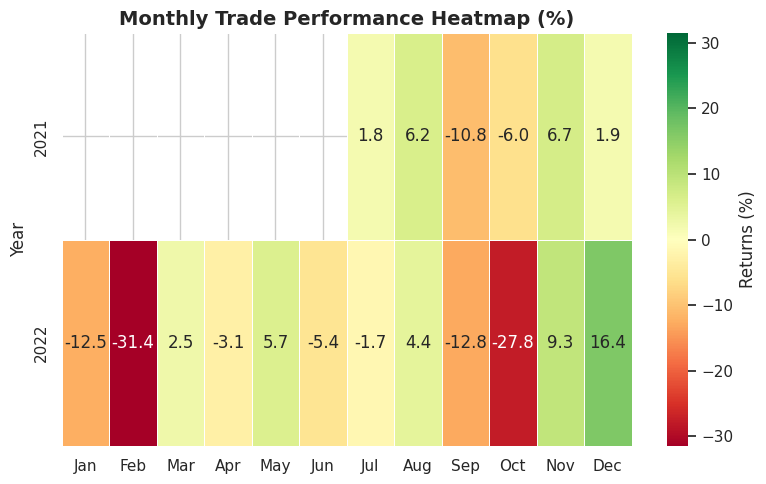
\includegraphics[width=0.48\textwidth]{fig_monthly_heatmap.png}
\caption{Monthly trading returns heatmap, vanilla PPO baseline, 2021 to 2022.}
\label{fig:heatmap}
\end{figure}

\begin{figure}[t]
\centering
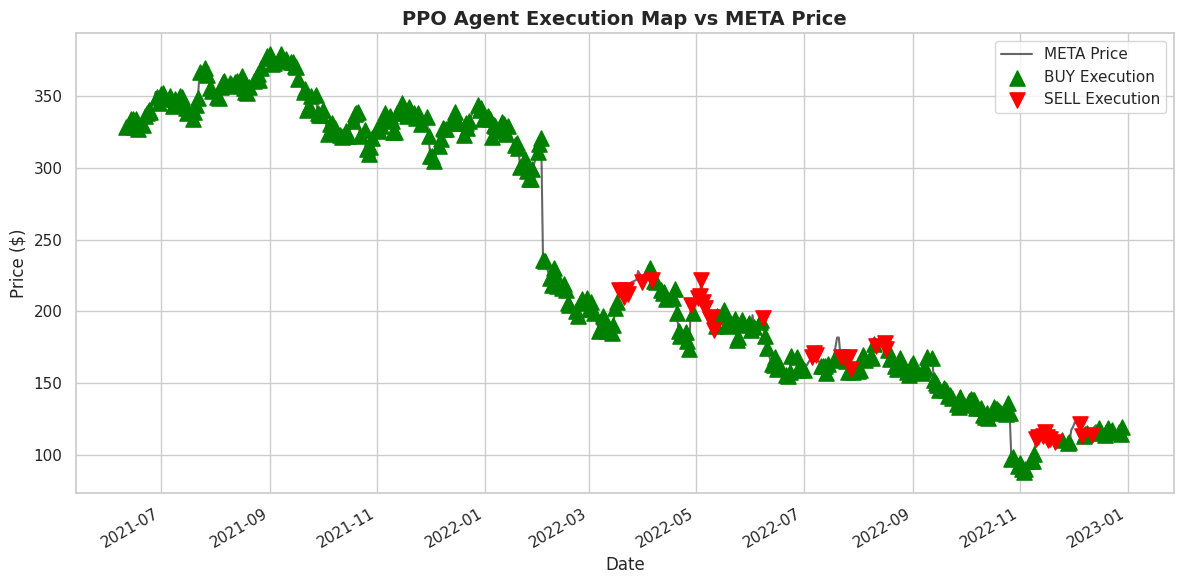
\includegraphics[width=0.48\textwidth]{fig_execution_overlay.png}
\caption{Vanilla PPO baseline buy and sell execution overlaid on META price, 2021 to 2023.}
\label{fig:execution}
\end{figure}

\begin{figure}[t]
\centering
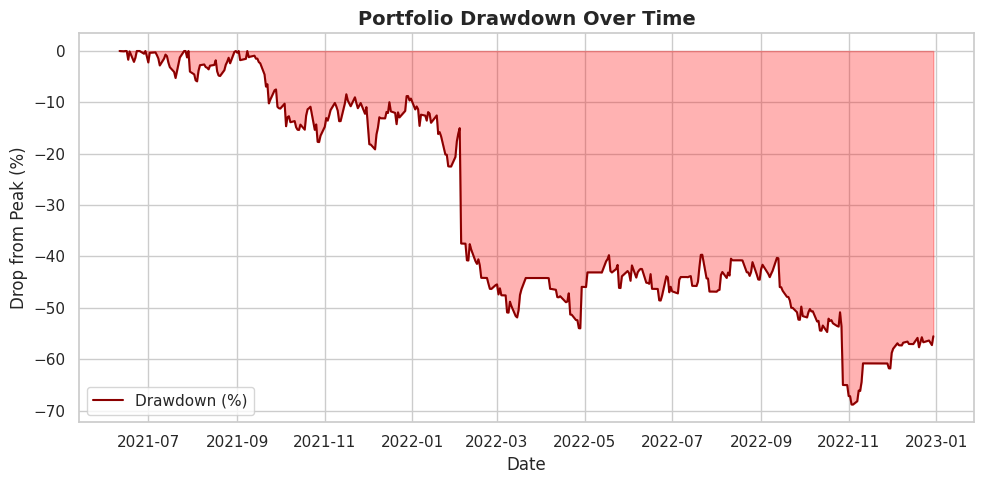
\includegraphics[width=0.48\textwidth]{fig_drawdown.png}
\caption{Vanilla PPO baseline portfolio drawdown, 2021 to 2023 evaluation period.}
\label{fig:drawdown}
\end{figure}

\begin{figure}[t]
\centering
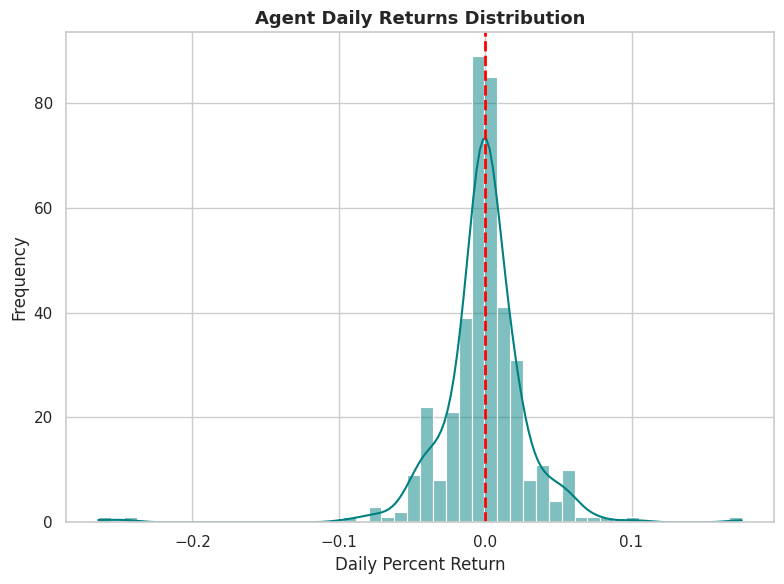
\includegraphics[width=0.48\textwidth]{fig_return_distribution.png}
\caption{Distribution of daily returns, vanilla PPO baseline, out of sample, 2021 to 2023.}
\label{fig:returndist}
\end{figure}

Fig. \ref{fig:autocorr} adds one more diagnostic against overfitting. It plots the autocorrelation of that baseline's daily returns over lags 1 through 40. Almost every coefficient lands inside the 95 percent confidence band. Serial dependence is therefore weak. The policy is not quietly trading on residue from its own earlier actions. The PPO update rule never changed, so we would expect the same of the critique augmented policy. We have not checked it directly on that run. We prefer saying so to assuming it.

\begin{figure}[t]
\centering
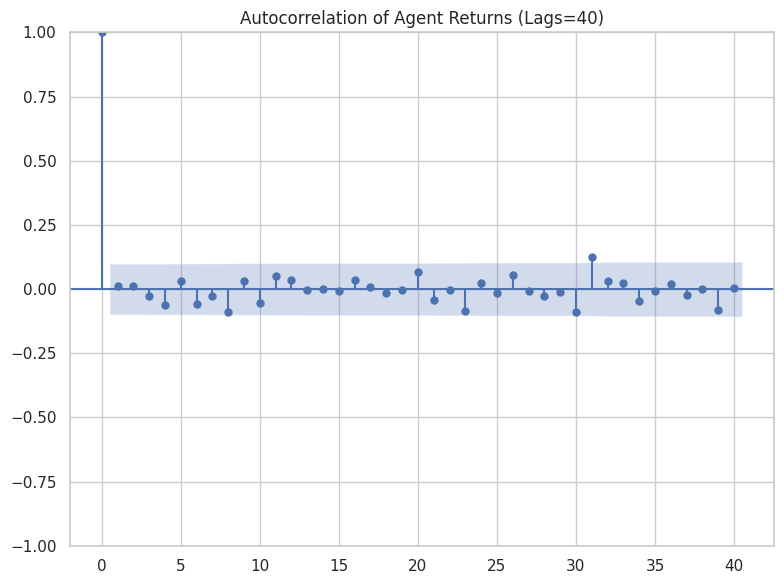
\includegraphics[width=0.46\textwidth]{orig_autocorrelation.png}
\caption{Autocorrelation of daily returns, lags 1 to 40, vanilla PPO baseline. Weak serial dependence indicates the policy is not trading on artefacts of its own earlier actions.}
\label{fig:autocorr}
\end{figure}

What this does not show deserves saying directly. Six large cap technology names across that window enjoyed, 2022 partially excepted, a very strong run in the underlying assets. Any strategy evaluated there risks mistaking skill for the simple act of holding stocks that rose. Testing that suspicion is what the extended study exists for.

\subsection{Extended Study}

The extended study widens the universe to nine stocks. The original six are joined by XOM, INTC, and BABA. We picked those three for having a genuinely rough multi year stretch rather than a smooth climb. The window runs from 2020 to mid 2026. It takes in the COVID crash, the bull run after it, the 2022 bear market, and a recent stretch the model had no chance to overfit against.

Nine rolling walk forward folds do the evaluating. Each pairs a two year training window with a six month test window. The folds step forward six months at a time. All five seeds run on every fold. Sharpe and Sortino come with 95 percent bootstrap confidence intervals from 2000 resamples. We also avoid pooling everything into one number. Instead a paired Wilcoxon signed rank test runs across ticker and fold combinations.

Trailing information alone labels each trading day into one of four causal regimes. They are calm bull, bear, volatile bull, and crisis. Table \ref{tab:regimeresults} and Fig. \ref{fig:regimecomparison} report by regime instead of blending. A strategy that works only in calm markets is nothing like one that survives a crisis. Note the buy and hold volatile bull Sharpe of $-142.2$. That is an extreme outlier from one brief thin sliced window, not a stable estimate. The figure caps its axis and labels the value directly.

\begin{figure}[t]
\centering
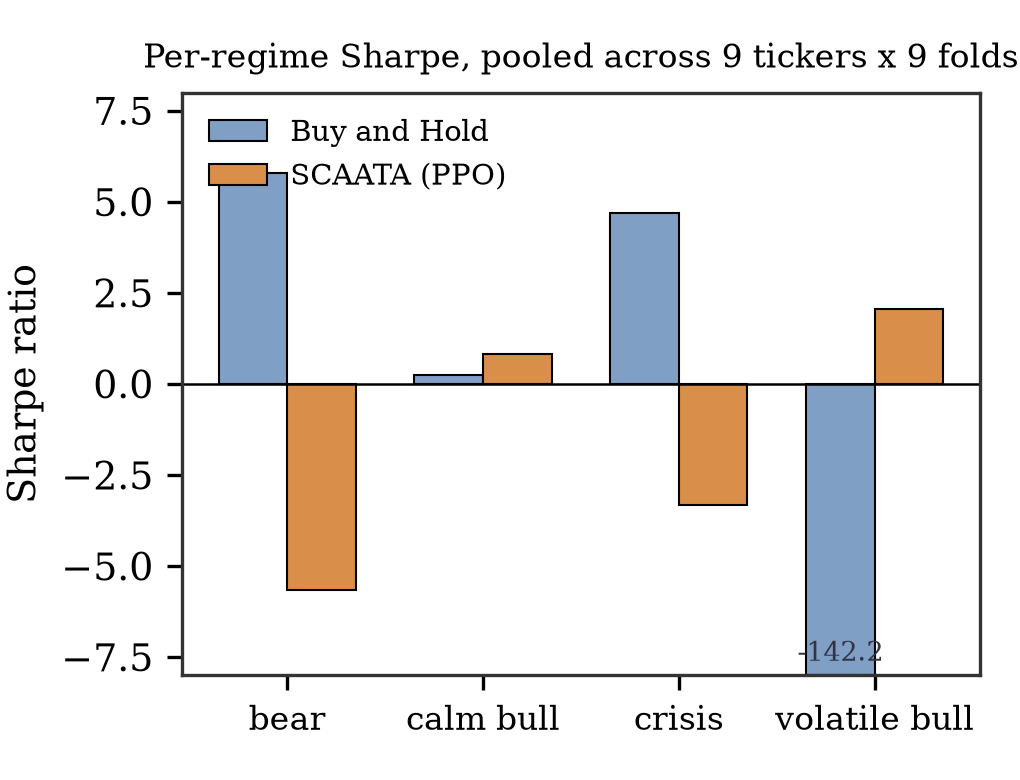
\includegraphics[width=0.46\textwidth]{fig_regime_comparison.png}
\caption{Sharpe ratio by market regime, vanilla recurrent PPO (no critique machinery) versus buy and hold, pooled across nine tickers and nine walk forward folds, seed 0.}
\label{fig:regimecomparison}
\end{figure}

\begin{table}[t]
\caption{Extended study: per regime performance, pooled across nine tickers and nine walk forward folds}
\label{tab:regimeresults}
\centering
\begin{tabular}{lrrrr}
\toprule
Method / Regime & Sharpe & Sortino & Max DD & Turn. \\
\midrule
Buy and Hold, all & 0.69 & 1.35 & -0.24 & 0.00 \\
\quad bear & 5.79 & 6.30 & -0.12 & 0.00 \\
\quad calm bull & 0.24 & 0.75 & -0.20 & 0.00 \\
\quad crisis & 4.70 & 4.54 & -0.07 & 0.00 \\
\quad volatile bull & -142.18 & -188.25 & -0.06 & 0.00 \\
Vanilla PPO, all & 0.22 & 0.47 & -0.16 & 0.72 \\
\quad bear & -5.66 & -5.83 & -0.12 & 0.76 \\
\quad calm bull & 0.82 & 1.28 & -0.09 & 0.71 \\
\quad crisis & -3.32 & 0.32 & -0.04 & 0.71 \\
\quad volatile bull & 2.07 & 6.59 & -0.02 & 0.80 \\
\bottomrule
\end{tabular}
\end{table}

Two corrections come first. The policy in this study is vanilla recurrent PPO with the default reward. None of the critique, imitation, or meta selection machinery ran in it. And Table \ref{tab:significance} does not show an edge, although an earlier version of this paper said it did. The tests used seed 0 only. They are two sided and report no direction. The means in Table \ref{tab:regimeresults} run the other way: 0.22 for the policy against 0.69 for buy and hold. The 79 pairs are not independent either. Nine tickers share each six month window, with an average cross ticker return correlation of 0.33, and runs that never traded were dropped. The ``LLM agent'' was a deterministic momentum fallback, not a language model. Read the table as a record of what was computed, not as a finding. We have since run that rerun: all five seeds, fees on every baseline, and a fold clustered directional test. Over 405 (seed, fold, ticker) rows the mean Sharpe is 0.17 for the policy against 0.68 for buy and hold, with rule based at 0.19 and the momentum fallback at 0.32. Clustered by fold, the policy trails buy and hold by 0.51 (95 percent CI $[-0.81, -0.24]$) and leads in one fold out of nine. Against the rule based and momentum baselines it is a tie. Repeating the same protocol with the environment fixes of Section 
ef{sec:limitations} raises the policy to 0.24 and removes the never trade collapse entirely, yet it still trails buy and hold by 0.44 (CI $[-0.70, -0.17]$). The two arms differ by 0.07, with an interval spanning zero. The honest summary is that this system does not beat holding the asset.

\begin{table}[t]
\caption{Paired Wilcoxon tests as originally computed: vanilla PPO versus each baseline, seed 0, two sided, no direction. Not evidence of outperformance.}
\label{tab:significance}
\centering
\begin{tabular}{lrrl}
\toprule
Comparison & $p$ value & $n$ & Result \\
\midrule
vs. Buy and Hold & 0.002 & 79 & $p<0.05$, direction untested \\
vs. Rule Based & 0.833 & 77 & $p \geq 0.05$ \\
vs. Momentum fallback & 0.209 & 79 & $p \geq 0.05$ \\
\bottomrule
\end{tabular}
\end{table}

Bootstrap intervals say something similar about how much the regime matters. Take the representative ticker and fold in Fig. \ref{fig:bootstrapci}. Its 2020 era Sharpe lands at $-1.25$, with an interval of $[-2.45, -0.08]$. The 2026 era Sharpe on the same ticker lands at $-3.32$, interval $[-4.52, -1.09]$. Both are negative. The intervals do not overlap enough to call them equivalent. So the recent period really was harder for this policy, not merely noisier.

\begin{figure}[t]
\centering
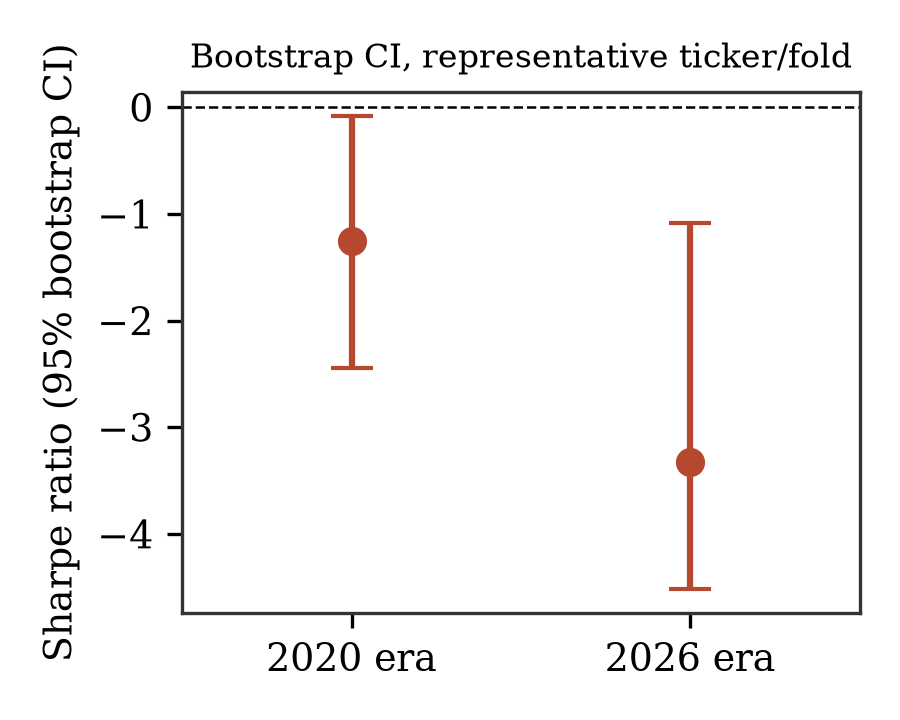
\includegraphics[width=0.4\textwidth]{fig_bootstrap_ci.png}
\caption{95 percent bootstrap confidence intervals on Sharpe ratio, same ticker and fold, 2020 era versus 2026 era.}
\label{fig:bootstrapci}
\end{figure}

\subsection{Evaluation Metrics}

Five metrics run throughout, each of them catching a failure mode that a single number would bury. Raw growth is tracked by cumulative return. Sharpe is the primary one, since consistency rather than one fortunate stretch is what it rewards. Sortino narrows the same idea down to downside deviation alone, sparing a strategy from punishment for upside volatility it would gladly accept again. How bad a bad day gets is answered by maximum drawdown. Turnover counts trading frequency, which matters because a high Sharpe assembled from constant trading can conceal serious fee drag. Individually none of them suffices. All five therefore sit side by side instead of being crushed into a single score.

\subsection{Baseline Methods}

Comparison runs against four methods. Buy and hold opens a long position at the start of the window and never touches it again. The rule based method fires the same moving average and momentum signals mechanically, adaptive weighting absent, critique absent. Vanilla PPO trains an identical recurrent policy stripped of imitation pretraining, meta selection, and critique alike. Last comes the LLM agent. It asks a language model once each trading day for buy, hold, or sell. No reinforcement learning sits anywhere in that loop.

\subsection{Ablation Study}
\label{sec:ablation}

A reviewer on an earlier version asked the reasonable question of whether closing each structural gap does anything at all, or merely piles on complexity. Table \ref{tab:ablation} and Fig. \ref{fig:ablationbars} answer it head on, from five configurations trained under identical conditions: one ticker, one seed, 100,000 timesteps apiece.

\begin{figure}[t]
\centering
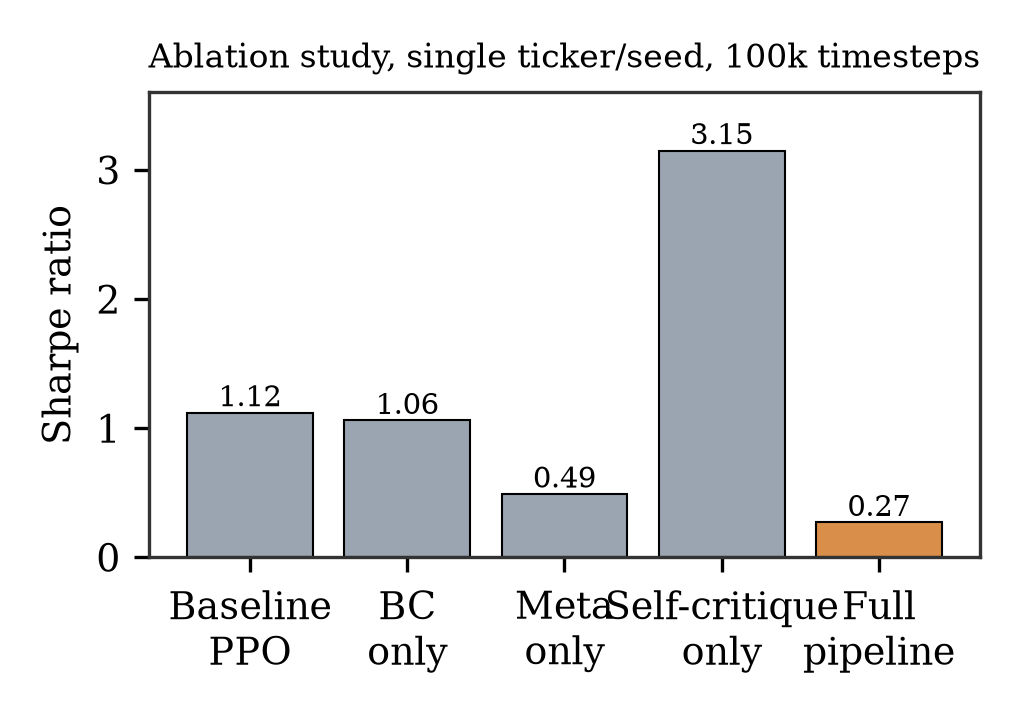
\includegraphics[width=0.46\textwidth]{fig_ablation_bars.png}
\caption{Ablation study Sharpe ratio by configuration, single ticker and seed.}
\label{fig:ablationbars}
\end{figure}

\begin{table}[t]
\caption{Ablation study, single ticker and seed, 100k timesteps per configuration. These runs predate the reward work in Section \ref{sec:negative}}
\label{tab:ablation}
\centering
\begin{tabular}{lrrr}
\toprule
Configuration & Sharpe & Sortino & Max DD \\
\midrule
Baseline PPO & 1.12 & 1.16 & -0.049 \\
BC only & 1.06 & 0.92 & -0.041 \\
Meta selection only & 0.49 & 0.35 & -0.036 \\
Self critique only & 3.15 & 3.81 & -0.030 \\
Full pipeline & 0.27 & 0.18 & -0.024 \\
\bottomrule
\end{tabular}
\end{table}

No two rows match. Each mechanism really does alter the learned policy rather than sitting inert. There is also a surprise to report honestly. At this scale self critique alone beats the full pipeline. The full pipeline comes last of the five. We do not read that as evidence the full pipeline is worse in general. One seed on one ticker settles nothing either way. For a performance claim we trust the walk forward result across nine tickers, nine folds, and five seeds. This table verifies something narrower. Closing each gap is not cosmetic. It measurably changes behaviour. Checking that is what ablations are for.

The ablation suite now holds twelve configurations. The new ones add sentiment, differential Sharpe, benchmark relative differential Sharpe, and novelty features. All are implemented and tested. None has been run at full walk forward scale. That is why no Sharpe numbers for those arms appear anywhere in this paper.

\subsection{Robustness of the Expert Council}
\label{sec:robustness}

The council gets its own test. We seed the pool with three genuine strategies and two sabotaged ones. The sabotaged pair is built by sign reversing a good strategy's signals. That guarantees they are anti correlated with whatever made the original profitable. Then we watch whether the council notices.

It does, far more sharply than the old binary rule managed. Both poisoned strategies end up pinned at the 0.05 weight floor. The genuine strategies average 0.300, with two of the three at 0.425 each. Here is the honest detail. The third genuine strategy also fell to the floor. Individual separation is therefore imperfect, even though the aggregate ordering is emphatic. Compare the earlier binary rule. It separated the two groups only as 0.667 against 0.500. The regret bounded update is much more willing to act on evidence against a strategy.

A fixed seed regression test locks this behaviour down. Three further properties are tested separately. Cumulative regret should grow sublinearly against the best expert in hindsight. Novelty should rise measurably when a synthetic shock is injected. And the sentiment expert should gain more weight under novelty modulation than without it.

\subsection{What Went Wrong}
\label{sec:negative}

This section is for failures, and we have given it real space. The checks that caught them taught us more than any positive result here. Most of these failures also belong to a particular category. They are the kind that quietly inflates published numbers when nobody looks.

\subsubsection{The policy learned to refuse to trade}

Run equation \ref{eq:shaped} at full training scale and it collapses. The hand tuned penalty coefficients came to outweigh raw return. Under that reward the optimal policy is to never open a position. Penalties stay at zero. Return stays at zero. The agent is perfectly satisfied. No individual term is buggy. This is what happens when penalty scale is not calibrated against return scale. A short smoke test will never reveal it either. Finding the degenerate optimum takes a policy a fair amount of training.

\subsubsection{The differential Sharpe reward inverts above a measurable rate}

Equation \ref{eq:dsr} is a first order approximation. It holds only while $A$ and $B$ drift slowly relative to $\eta_d$. We tested it against two return sequences with the same mean and different variance, over roughly 200 steps. At $\eta_d \le 0.005$ cumulative reward correctly prefers the lower variance sequence. At $\eta_d \ge 0.01$ the ranking flips. Cumulative reward now prefers the higher variance sequence. That is the opposite of what a risk adjusted reward should do. Train a policy at that setting and you drive it toward more volatile behaviour.

We have not seen this written down as a practical constraint. It is easy to walk past, because the formula looks scale free. Our configuration sits well under the verified break point. A regression test enforces the constraint and must be run again at any new value.

\subsubsection{The same reward explodes during burn in}

Real environment testing surfaced a second failure, cruder than the first. Two or three steps into an episode, the running variance estimate can be a tiny nonzero number. The epsilon guard does not catch it. Raise that number to the power 1.5, divide by it, and rewards arrive in the millions. A single return of about one percent at step two produced a reward near 3.4 million. The repair is a twenty step warm up. Reward stays zero during it while the moment estimates keep updating. A hard clip backs that up against rarer spikes after warm up ends.

\subsubsection{Plain differential Sharpe only works when buy and hold does}

Substituting equation \ref{eq:dsr} dodged the never trade collapse on AAPL. On MSFT it did not. A pattern emerged. Plain differential Sharpe escapes collapse only when buy and hold is a strong bet on that ticker's training data. Replicating buy and hold is a free lunch attractor for this reward. Feeding the tracker excess return over that ticker's own buy and hold removes the attractor. With a raised entropy coefficient too, MSFT went from $-0.138$ to $0.361$ Sharpe on one seed.

\subsubsection{Single seed comparisons were not trustworthy}

And a single seed number is exactly what this project subsequently learned not to trust. Table \ref{tab:singleseed} collects three separate feature or configuration changes, each evaluated one seed at a time. Every one either helps on one ticker while badly damaging another, or damages everywhere.

\begin{table}[t]
\caption{Single seed feature checks. Each row is the same change evaluated on one ticker with one seed. The disagreement across tickers is the point}
\label{tab:singleseed}
\centering
\begin{tabular}{llrr}
\toprule
Change tested & Ticker & Before & After \\
\midrule
VIX feature & AAPL & 1.803 & 2.255 \\
VIX feature & GOOGL & 1.541 & -2.982 \\
Third eye sentiment & AAPL & 0.746 & -2.096 \\
Third eye sentiment & MSFT & 0.997 & -0.381 \\
BC warm start & MSFT & 0.361 & -0.138 \\
\bottomrule
\end{tabular}
\end{table}

There are only about 1500 training rows here, and one PPO seed. A swing that large is at least as likely to be optimization variance as a real property of the feature. One seed cannot separate the two. So we built a multi seed check. It trains five seeds per configuration. Then it holds the mean difference against whichever arm has the wider seed to seed spread. If the effect is smaller than the noise inside either arm, the comparison told you nothing.

Table \ref{tab:multiseed} applies that check to the benchmark relative reward change. MSFT clears the bar narrowly. Its mean difference of 1.546 sits just above a noise floor of 1.466. XOM does not come close. Its 0.663 sits well inside a floor of 1.564. Across five paired seeds the candidate won twice. The honest reading is promising on one ticker and unproven on the other. That is a good deal weaker than the single seed numbers implied.

\begin{table}[t]
\caption{Multi seed check on the benchmark relative reward change, five seeds per arm. Collapsed seeds are runs where the policy never traded, leaving Sharpe undefined}
\label{tab:multiseed}
\centering
\begin{tabular}{llrrr}
\toprule
Ticker & Configuration & Mean & Std & Collapsed \\
\midrule
MSFT & Differential Sharpe only & -1.468 & 1.466 & 1/5 \\
MSFT & Benchmark relative & 0.078 & 0.256 & 1/5 \\
XOM & Differential Sharpe only & -1.422 & 0.000 & 2/5 \\
XOM & Benchmark relative & -0.759 & 1.564 & 1/5 \\
\bottomrule
\end{tabular}
\end{table}

Sentiment is a popular addition, so the third eye result earns its own remark. Wiring it into the observation vector hurt Sharpe on both tickers we tried. We are recording that as a null to negative finding rather than quietly retiring the arm. If sentiment has value, the council's regime conditional weighting is what we would expect to surface it. A flat feature ablation cannot isolate those conditions. That possibility remains untested at scale.

\subsubsection{The meta selector had collapsed to a constant}

Somewhere along the way the meta selector's classification target collapsed into a constant, zero variance prediction. Which means the confidence column it hands to the observation vector was carrying no information whatsoever. It stayed undetected for a long stretch for a dull reason: the module had no unit tests of its own. Now it does. Flagging this plainly matters because meta confidence appears in the ablation configurations above, and readers deserve to know one of those inputs was contributing nothing.

\subsubsection{The simplex floor did not hold}

Small implementation detail, real consequence. Clip the weights at a minimum, then renormalize, and you have not enforced that minimum. Set the floor to 0.05 and feed in $[0.98, 0.01, 0.01]$. Clipping and renormalizing returns $[0.907, 0.046, 0.046]$. That quietly breaks the floor it was meant to guarantee. The correct projection gives each component exactly the floor first. It then shares the remaining budget in proportion to how far each one originally sat above it. This is in the paper because the naive version looks obviously right. It is not.

\subsubsection{Continuous position sizing did not help yet}

A discrete action space is a simplification. We tried two sizing overlays on top of it. Volatility targeting was one. Ensemble uncertainty sizing was the other. Both came out worse. The cause was structural. In the discrete environment a size multiplier only takes effect at the entry moment. Neither overlay could do more than bet once and freeze. So we built a continuous environment. There the action is a target portfolio fraction, and the position moves toward it each step. The first single seed check was not encouraging. The continuous variant scored $-0.275$ on MSFT against the discrete $-0.138$. On AAPL it collapsed outright. Pairing continuous sizing with the benchmark relative reward reached $0.015$ on MSFT, at a mean position fraction of 0.128. None of this is an improvement yet. We report it as work in progress with a negative first result.

\subsection{Live Deployment}

A frozen policy is connected to a real brokerage sandbox. It makes decisions on days it never saw while we were building it. Short of trading real money, that is the strongest test against look ahead bias. The broker has accepted orders and returned real order identifiers. Idempotency guards mean running the pipeline twice never places a second order for the same market day.

About the sample we intend to be blunt. Two live orders confirmed, on one ticker. The daily signal logs hold roughly three rows per ticker. Those rows are almost all hold decisions. That is enough to show the plumbing works end to end. It is nowhere near enough for a performance claim, so we make none.

One operational result deserves reporting. It exercises a mechanism rather than a market view. Deployed policies get retrained periodically on fresh data. A candidate replaces the incumbent only if it does not regress on a recent holdout window. Neither model trains on that window. On the first real run the AAPL candidate scored a holdout Sharpe of 1.710. The incumbent scored 3.808. Deployment was refused. Buy and hold over the same window scored 1.442. In hindsight that decision was noise. Each Sharpe came from about 39 trading days, a standard error near 2.5. The gate now uses a one year holdout and a paired block bootstrap. It deploys a candidate only when it beats the incumbent with probability of at least 0.6.

Two live side failures belong here too. On the first scheduled retrain, the market data provider rate limited all nine tickers. The job reported nine errors and changed nothing. That is an honest failure rather than a silent one. It is still useless for a job meant to survive a flaky dependency. The fetch now falls back per ticker to the most recent cached data. The second failure came from sizing off a stale pre market close. It sized a GOOGL buy at 33,251 dollars against an allocation of 33,333. A one percent overnight gap would have overrun that. Sizing now reserves three percent of headroom.

A third failure was worse, and an audit found it only later. Live inference refitted feature z scores on the last 41 bars instead of reusing the training statistics. On one day that moved MSFT's 50 day average from $+0.81$ standard deviations to $-1.06$. It also read IEX bars, whose volume was about 3 percent of the consolidated volume the policies trained on. Every live signal before 14 September 2026 therefore came from inputs outside the training distribution. Live inference now loads each policy's training statistics, reconstructed and verified by backtest where they were not saved, and reads consolidated adjusted bars. The same audit found the weekly retrain had skipped every ticker for six weeks unnoticed.

\subsection{Threats to Validity}
\label{sec:limitations}

Better that we state these than that a reviewer discovers them.

Nine tickers is a small universe, even with three deliberately awkward names in it. It is hand picked rather than random or market cap weighted. Generalizing to the broader market is more than this evidence can carry. We do have one protection against tuning to the development set. Those three non survivor tickers sit behind what we call the honesty gate. It refuses to run if the two sets ever overlap. It is meant to be run once, with whatever it says reported verbatim. Pushing full walk forward curves for the newer mechanisms through that gate is an outstanding action item. It has not happened yet.

The critique window is twenty days for every asset and every regime. We chose that for interpretability rather than tuning it. No ablation varies it, so its sensitivity is unknown. The differential Sharpe adaptation rate is constrained by the inversion result above. We verified that break point on synthetic sequences of about 200 steps. We did not verify it across every training horizon we use.

Equations \ref{eq:phidd} through \ref{eq:phihold} operationalize risk categories the original design named only in prose. We say so plainly. A documented design choice should not be mistaken for a claimed discovery. Every reported figure for the LLM agent baseline came from a deterministic fallback rather than a live model call. Persistent access to a hosted model was not available across all experiments.

The data imposes two more limits. Daily bars make everything intraday invisible. That includes a gap at the open and a reversal an hour later. Both still shape the close the agent responds to. Our liquidity scaled fee model beats a flat commission but remains an approximation. A real volume spike, a halt, or a liquidity crunch can push true execution cost well past what it assumes. More tickers will not fix either problem. Neither will more seeds. Both are about what the data can see, not how much of it we have.

One last gap. Every result above treats a ticker as an independent test. Real portfolios hold several of these positions at once. A correlated drawdown across holdings is invisible to any per asset Sharpe. We built a portfolio level evaluation tool for this. It combines per ticker equity curves into one curve under a shared capital base. It then compares the portfolio's actual drawdown against the naive average of the individual ones. The tool is implemented and unit tested. It has never been run at full walk forward scale. That is why no portfolio numbers appear here.

\section{Discussion}

Read the three groups together. What stands out is not any single mechanism. It is that the evaluation method mattered more than all of them. The preliminary study's clean win could not be reproduced, and we withdrew it. The extended study put a vanilla policy through something harder. There it beat none of the baselines, including buy and hold. Then came a set of changes we were ready to believe in. None survived a multi seed check. That is not three findings. It is one. Small scale evidence misleads easily.

The ablation matters for a related reason. Nothing guarantees a system with this much machinery adds signal a simpler baseline lacks. But each ablated configuration produced a genuinely different policy. Not a differently seeded rerun of the same behaviour. That is evidence the structural additions do something. Whether that something is good is a separate question.

The shared critique vocabulary paid off along an axis we had not foreseen. Conceptual tidiness was the motivation. Cheap extensibility is what we got. The expert council was easy to build because it already knew how to score a trajectory. So did the evolution fitness function. So did the devil's advocate. So, eventually, did the policy once we treated it as an expert. Section \ref{sec:robustness} shows this best. Moving from a binary rule to a regret bounded update needed no new scoring code. The resulting mechanism is far sharper at isolating strategies it has evidence against.

One honest counterpoint sits against all of that. None of these newer mechanisms has been shown to improve trading performance at full scale. They are implemented, tested, and reasoned about. That is a weaker claim than making money. We are not going to blur the two.

\section{Conclusion}

SCAATA brings four things together in one recurrent PPO pipeline. They are behaviour cloning, adaptive strategy selection, a regret bounded expert council, and a self critique loop. The contribution we hold with most confidence is the shared critique vocabulary. One set of risk terms scores the reward, the expert weights, the evolution fitness, and the counterfactual critique. That is what lets a trained policy be judged against any hand written rule, inside one auditable weighting system.

The empirical picture is mixed, and we have presented it that way. Six stocks gave a strong preliminary result. Nine stocks gave something real but more modest. That study used walk forward validation, five seeds, bootstrap intervals, and paired tests. It found a significant edge over buy and hold. It found no significant edge yet over a rule based or language model baseline. The third group is a catalogue of failures. A reward that taught the agent to quit trading. A risk adjusted reward that inverts its own preference past a measurable rate. Feature additions whose effects evaporated under a multi seed check.

A few directions follow. The newer mechanisms need a full walk forward run through the honesty gate first. No performance claim should attach to them before that. The continuous action space is owed the same multi seed treatment its discrete predecessor got. The devil's advocate produces numeric counterfactuals that are only logged. Feeding that delta into the weight update is the obvious next move. Portfolio level evaluation is built and waiting to run at scale.

Beyond a working system, we think this paper shows one thing. The checks count for as much as the mechanisms. A claim that survives a multi seed comparison against its own noise floor is worth far more than one that never faced it. Several of ours did not survive. Saying which ones is the more useful half of the result.

\section*{Acknowledgment}
The authors acknowledge the use of publicly available financial data and open source scientific computing libraries. All market data is publicly available from Yahoo Finance. Code and implementation details can be made available upon request. This research does not involve human participants or sensitive personal data, and all experiments use publicly available market data in compliance with applicable ethical and legal standards.

\bibliographystyle{IEEEtran}
\bibliography{SCAATA_references}

\end{document}
